\chapter{Architectural Design}


\section{Architectural Overview}

\subsection{Interactive subsystem (Type)}

The mobile app allows the ranger to perform specific actions, such as:
\begin{itemize}
	\item Connecting to the drone
	\item Giving basic commands to the drone
	\item Viewing the detections
\end{itemize}
This is done because the ranger may be required to connect to multiple drones and have the ability to communicate with each indepenently.

\subsection{Event driven system (Type \& Style)}

\begin{itemize}
	\item Object recognition notifies the server based on object detections made in real time. 
	The server will process this information and decide whether or not an event has been triggered. 
	If it has, then it will emit a signal to the mobile app notifying it of a detection.

	\item The server will be notified by the app of any ranger movements. The server will then issue 
	commands to the drone which will cause the drone to follow the ranger.
\end{itemize}
This was done because the drone needs to change its actions based on actions. Our systems need to change their behaviour
based on specific inputs and adjust accordingly.

\subsection{Database system (Type) \& persistence (Style)}

\begin{itemize}
	\item Dropped pins generated from server snapshots will contain animal snapshots, location data and drone information. 
	These pins will be stored in a database for future use.
\end{itemize}
This is done in order to record data for any future use that may be required.

\subsection{Client-server}

\begin{itemize}
	\item At the centre of our system we have a server that acts as a mediator. The clients, object recognition and the mobile app, 
	communicate back-and-forth with the server, relaying information as events are triggered.
\end{itemize}
We have multiple subsystems that need to communicate with each other, thus a central server with multiple clients was the ideal solution.
The server also allows us to open a socket between it and the app, allowing data to be pushed instead of needing to poll.

\section{Design Principles}

\begin{itemize}
	\item Due to separation of concerns, high cohesion and modular design, our system is implemented in such a way as to be easily changed in the future.
	Thus implying a design for changeability, maintainability and upgradeability.
	\item The subsystems are designed to be general purpose, to allow for repurposing if need be. 
\end{itemize}

\section{Deployment Diagram}

\begin{sidewaysfigure}[h!]
    \centering
		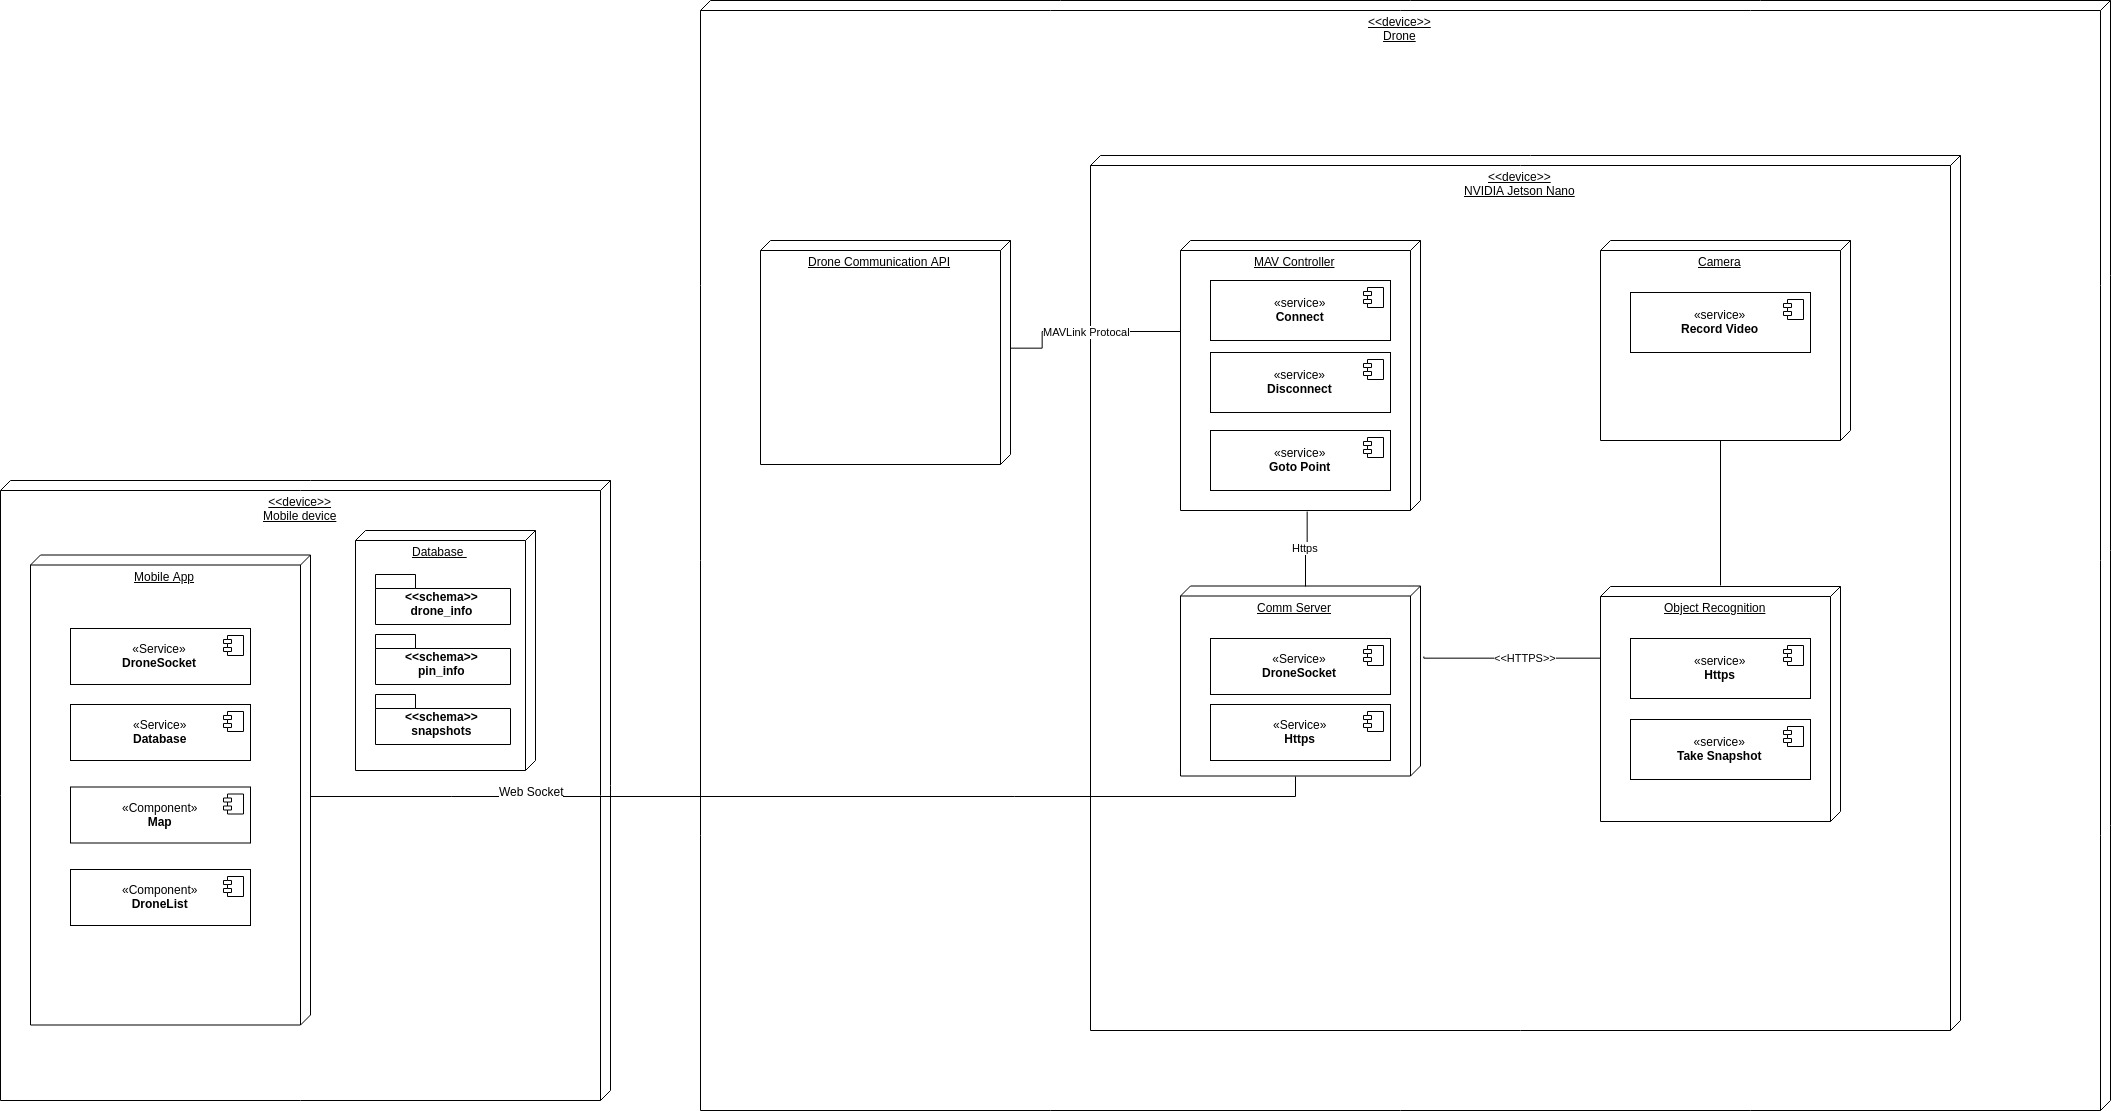
\includegraphics[scale=0.3]{./assets/images/deployment-diagram.jpg}
    \label{fig:awesome_image}
\end{sidewaysfigure}
	% \begin{figure}[h!]
	% 	\centering
	% 	\label{fig: erp-logo}
	% 	\caption{}
	% \end{figure}

